% !TeX spellcheck = en_GB
\def\ChapterTitle{Comparative Analysis of Multi-Domain Trust Assessment in Collaborative Marine MANETs}

\ifx\ifthesis\undefined
\documentclass[a4paper, 11pt]{article}

% % Special Includes stolen from Thesis.cls
\usepackage{booktabs}
\usepackage{hyperref}
\usepackage{graphicx}
\usepackage{epstopdf}
\usepackage{subcaption}
\usepackage{rotating}
\usepackage{listings}
\usepackage{lstpatch}
\renewcommand{\arraystretch}{1.3}

% % % % % % % % % % % % % % % %

% PACKAGES
\usepackage[square, numbers, comma, sort&compress]{natbib}  % Use the "Natbib" style for the references in the Bibliography
\usepackage{verbatim,listings}  % Needed for the "comment" environment to make LaTeX comments
\usepackage{array}  % Needed for the "comment" environment to make LaTeX comments
\usepackage{vector}  % Allows "\bvec{}" and "\buvec{}" for "blackboard" style bold vectors in maths
\usepackage{amsmath,amsfonts,amsthm,color,psfrag,epsf, tabularx, multirow, longtable}
\usepackage{snapshot, todonotes}
% \usepackage{pstricks}
\usepackage{enumerate}
%\usepackage[lined,algonl,boxed]{algorithm2e}
\usepackage[ruled,linesnumbered,vlined]{algorithm2e}
\usepackage{float}
\usepackage{epigraph} % epigraph
\usepackage{tikz}
\usetikzlibrary{shapes.geometric, arrows}

\usepackage{setspace}
\doublespacing
% or:
%\onehalfspacing

% SETUP
\hypersetup{urlcolor=blue, colorlinks=false}  % Colours hyperlinks in blue, but this can be distracting if there are many links. 
\DeclareGraphicsExtensions{.pdf,.jpeg,.png}
\graphicspath{{../Figures/}{../../../Dropbox/Thesis_Figures/}}  % Location of the graphics files (set up for graphics to be in PDF format)

% NOTE THERES A FUCKUP IN TEX4HT http://tug.org/pipermail/tex4ht/2014q2/000944.html
% NEED TO MANUALLY CHANGE \def\pgfsys@svg@newline{{?nl}}
\ifdefined\HCode
\usepackage[compatibility=false]{caption}
\def\pgfsysdriver{pgfsys-tex4ht.def}
\else
\usepackage[]{caption}
\fi

% \SpecialCoor
\def\subsum{\mathit{\Sigma}}

%opening
\title{\ChapterTitle}
\author{Andrew Bolster}

\begin{document}

\maketitle

\else
\chapter{\ChapterTitle}
\label{Chapter\thechapter}
\lhead{Chapter \thechapter. \emph{Analysis of Multi-Domain Trust Assessment}} % Write in your own chapter title to set the page header
\fi

\section{Introduction}



In this chapter we demonstrate the use and operation of a multi-domain trust management framework (MD-TMF) in collaborative marine MANETS
We demonstrate a methodology that applies Grey Sequence operations and Grey Generators (conceptually analogous to Sequential Bayesian Filtering) to provide continuous trust assessment in a sparse, asynchronous metric space across multiple domains of trust.
We present a methodology for assessing the performance of varying metric sets in detection and differentiation of a range of communications and physical misbehaviours, demonstrating that by utilising information from multiple domains, trust assessment can be more accurate in identifying misbehaviour than in single-domain assessment.

The core part of this chapter was submitted to AAMAS 2016

\section{Construction of Multi-Domain Trust}

A key question in this chapter is to assess the advantages and disadvantages of utilising trust from across domains. 
This includes a secondary question as to how trust assessments from these domains are most effectively combined. 

It is important to clarify what is meant by ``effective'' in this case; we take the ``effectiveness'' of any trust assessment framework as consisting of several parts.

\begin{enumerate}
  \item the \emph{accuracy} of detection and identification of a particular misbehaviour
  \item the \emph{timeliness} of such detections
  \item the \emph{complexity} of such analysis, including any specific training required
  \item the \emph{commonality} of the results of any detections between perspectives (also termed ``isomorphism'' of results)
\end{enumerate}




\subsection{Communications Trust Metrics}

We use the same trust metrics from \cite{Guo2012} that are applicable to the marine environment, i.e. as the simulated modem stack does not operate on the same tiered data-rate approach as used in the 802.11 stack, that metric was not included. Remaining metrics are; Delay, Received and Transmitted power, Received and Transmitted Throughput, and Packet Loss Rate (PLR).

Thus, the metric vector used for communications-trust assessment is;

\begin{equation}
	X_{comms}=\{D, P_{RX}, P_{TX}, Tp_{RX}, Tp_{TX}, PLR\}
	\label{eq:comms_vector}
\end{equation}

\subsection{Physical Trust Metrics}

Three physical metrics are selected to encompass the relative distributions and activities of nodes within the network; Inter-Node Distance Deviation (INDD), Inter-Node Heading Deviation (INHD), and Node Speed. These metrics encapsulate the relative distributions of position and velocity within the fleet, optimising for the detection of outlying or deviant behaviour within the fleet.

Conceptually, INDD is a measure of the average spacing of an observed node with respect to its neighbours. INHD is a similar approach with respect to node orientation.

\begin{align}
	INDD_{i,j} &= \frac{|P_j - \sum_x \frac{P_x}{N}|}{\frac{1}{N}\sum_x \sum_y{|P_x - P_y| (\forall x \neq y)}}\\
	INHD_{i,j} &= \hat{v} \vert v= V_j - \sum_x{\frac{V_x}{N}}\\
	S_{i,j} &= |V_j|
\end{align}

Thus, the metric vector used for physical-trust assessment is;

\begin{equation}
  X_{phy}=\{\text{INDD}, \text{INHD}, S\}
	\label{eq:phys:vector}
\end{equation}

\subsection{Metric Weight Analysis Scheme}

From \eqref{eq:metric_weighting}, the final trust values arrived at are dependent on metric values, the weights assigned to each metric, and the structure of the $g$, $b$ comparison vectors.

This permits the assessment of the significance of different metrics in the detection and identification of different behaviours. 
For a metric weight vector $H$, where the metric $m_j$ is emphasised as being twice as important as the other metrics, we form an initial weighting vector $H'=[h_i...h_M]$ such that $h_i = 1 \forall i \ne j; h_j=2$. We then scale that vector $H'$ such that $\sum H = 1$ by $H= \frac{H'}{\sum H'}$.

The construction of the $g$ and $b$ vectors from \ref{eq:grc} depends on the particular metric, e.g. Throughput is positively correlated to trustworthiness and so follows the default construction ($g \mapsto \max, b \mapsto \min$).
However, in the case of a metric such as delay, this relationship is inverted, i.e. longer delays indicate less trustworthy activity.
In complex environments, the relationship between metrics trustworthiness correlations may not be quite so obvious as the throughput / delay examples.
This phenomenon was mentioned by Guo, but was manually configured for each metric for each behaviour and no analytical method for quantatively establishing such relationships has been presented since.

We include both the correlation and relevance of metrics to behaviours by signifying ``flipped'' metrics (i.e. those with the construction $g \mapsto \min, b \mapsto \max$) by a negative weight.

Using this process we can extract and highlight the primary aspects of an attack by comparing against the deviation from the ``fair'' result set, i.e. we are interested in the weight schemes that create the largest difference between fair and misbehaving cases.

With the nine selected metrics from across communications and physical behaviours, we can explore this metric space by varying the weights associated with each metric, and choose to emphasise across three levels; i.e. metrics can be ignored or over-emphasised. Naively this results in $3^9 = 19683$ combinations, however as these weights are being normalised, duplicates are introduced, e.g. $[0,0,0,0,1,0,0,0,0] \equiv [0,0,0,0,2,0,0,0,0]$ leaving 18661 unique weights for analysis.

To assess the performance of a given weight combination (i.e. an optimisation factor), we are initially interested in the metric weight vector that consistently provides the largest deviation in the final trust value $T$ across the cohort, i.e. producing the most clear detection of a node misbehaving in that particular fashion.
We approach this as an inverse outlier filtering problem, and select the range outside a $\pm\sigma$ envelope compared to the equivalent weighting in a known ``fair'' behaviour to assess detection (or comparing to other misbehaviours to assess discrimination). Note that at this point we establish ``signatures'' of different behaviours rather than optimal detection weights.

We apply a Random Forest regression \cite{Breiman2001} to assess the relative importance of the selected metrics on relative detectability of malicious behaviour. 
Random Forest accomplishes this by generating a large number of random regression trees and prune these trees to fit incoming data. A major advantage of Random Forest in this case is that by walking the most successful regression trees, we can acquire an already normalised maximal activation weight for the particular behaviour comparison being tested.

After establishing the importance of weights in particular behaviours, a final weight is arrived at by algorithmically those few metrics that are important, rather than having to further explore the computationally expensive weight-space.

Using this approach we can explore the results of these simulations, condensing the multi-dimensional problem (target / observer / behaviour / metric / time) down to a more tangible level for analysis.

\section{Results and Discussion}

\subsection{Significance Analysis}

First we discuss the results of the Random Forest regression assessment; in Figs~\ref{fig:comms_feature_extraction} and ~\ref{fig:phys_feature_extraction}, we show the resultant feature extraction signatures for Comms-only and Physical-only metric selections, and Fig~\ref{fig:multi_feature_extraction}, these metric spaces are brought together and reassessed.

It is also interesting to note that in both single-domain cases, there are clear 'signatures' in misbehaviours that don't directly target that domain ($P_{RX}$ in the Physical Shadow and Slowcoach behaviours in Fig~\ref{fig:comms_feature_extraction} and $INDD$ in the Selfish Target Selection behaviour in Fig~\ref{fig:phys_feature_extraction}).
This inter-domain activity is to be expected in MANETs in general, where the physical reality of the network (i.e. distance between nodes) directly impacts the behaviour of the logical communications network (i.e. delay between nodes), and is as we will see a useful characteristic for differentiating potential misbehaviours.



\begin{figure}[h!]
	\centering
  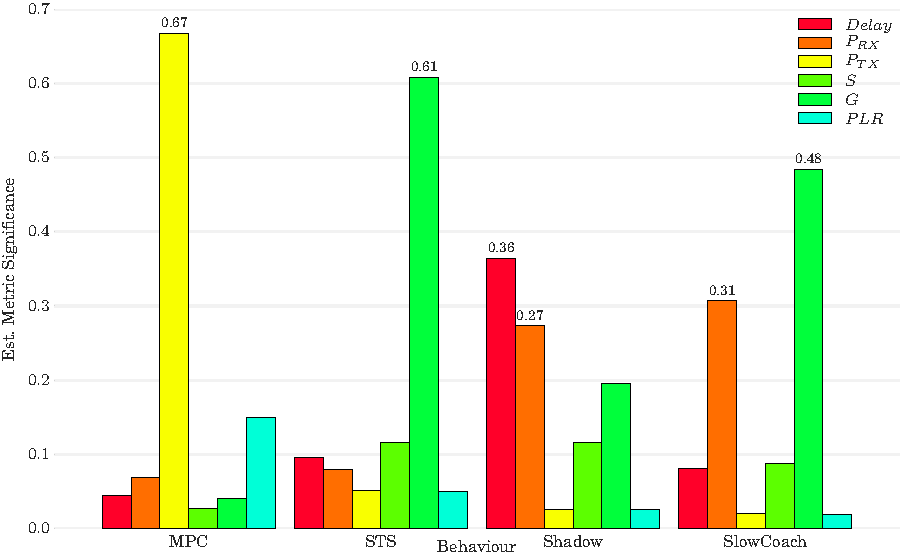
\includegraphics[width=\linewidth]{comms_metric_trust_relevance}
	\caption{Plot of $X_{comms}$ Metric Feature Extraction}
	\label{fig:comms_feature_extraction}
\end{figure}

\begin{figure}[h!]
	\centering
  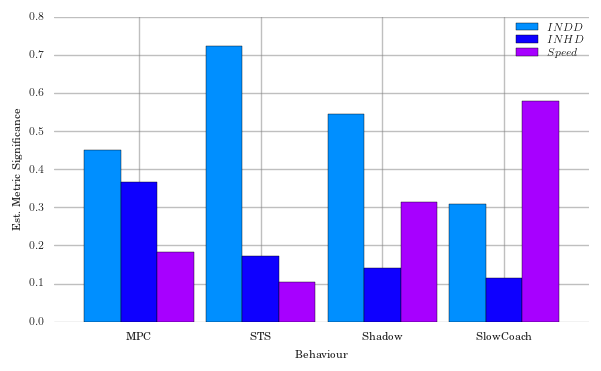
\includegraphics[width=\linewidth]{phys_metric_trust_relevance}
	\caption{Plot of $X_{phys}$ Metric Feature Extraction}
	\label{fig:phys_feature_extraction}
\end{figure}

\begin{figure}[h!]
  \centering
  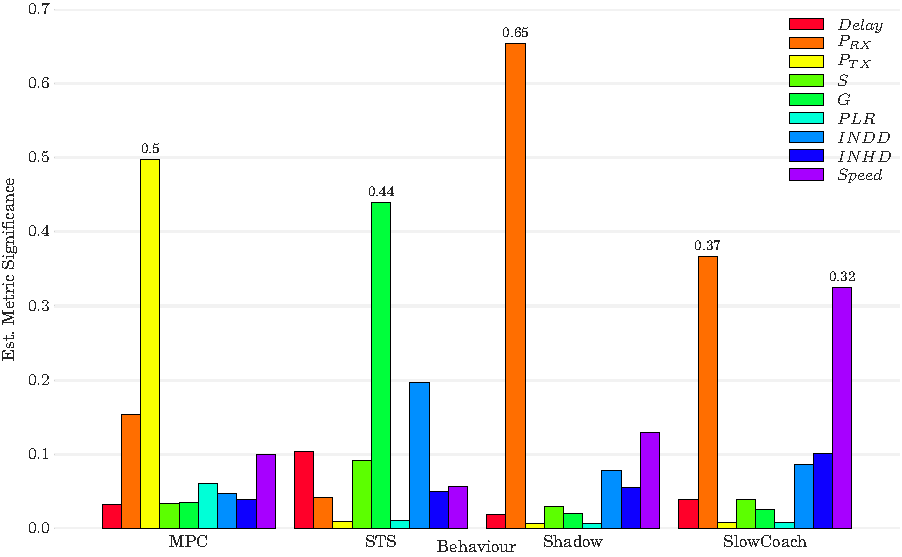
\includegraphics[width=\linewidth]{full_metric_trust_relevance}
  \caption{Multi Domain Relevance assessment of Metric Features}
  \label{fig:multi_feature_extraction}
\end{figure}

%\begin{tabular}{lrrrrrrrrr}
\toprule
{} &  $Delay$ &  $P_{RX}$ &  $P_{TX}$ &  $T^P_{RX}$ &  $PLR$ &  $T^P_{TX}$ &  $INDD$ &  $INHD$ &  $Speed$ \\
Misbehaviour &          &           &           &             &        &             &         &         &          \\
\midrule
MPC          &   -0.187 &     0.129 &     0.579 &       0.006 &  0.069 &      -0.146 &   0.040 &  -0.190 &   -0.297 \\
STS          &   -0.195 &    -0.035 &     0.019 &      -0.100 &  0.019 &       0.381 &  -0.209 &   0.057 &    0.062 \\
Shadow       &    0.004 &    -0.654 &     0.030 &      -0.016 &  0.030 &       0.063 &   0.120 &   0.158 &    0.266 \\
SlowCoach    &   -0.157 &    -0.533 &     0.013 &      -0.132 &  0.013 &      -0.028 &   0.159 &   0.206 &    0.460 \\
\bottomrule
\end{tabular}


\subsection{Weight Assessment}

From this significance information we can infer a signature for each behaviour, that can be fed back into the assessment framework, with the aim being to minimise the number of weight permutations required to come to a conclusion about the behaviour under observation. 

We take the feature significances as presented from the regression as baseline weight vectors, however, we have no algorithmically derived approach to the structure of the $g$,$b$ comparison vectors from \eqref{eq:metric_weighting}.

One option would be to go back to the regression point and expand the combination options to include negative values, however this is combinatorically explosive.
Instead, the ``significance'' weight is permuted against it's possible combinations of ``flips'', i.e. for $X_s=[0.3,0.4,0.01,0.02,0.27]$ could also be $X_s^p=[0.3,-0.4,0.01,0.02,0.27]$ and so on. 
This sign permutation is filtered based on a threshold value ($0.01$), so for all indices below that threshold will not be permuted on, halving the number of combinations required for each indices eliminated.

The best of these permutations is selected to both maximise the (correct) deviation between each nodes trust perspectives and to minimise the trust value reported for the misbehaving nodes; $\Delta T \max$

These weights are applied to untrained data to derive the following results.

An exemplar subset of the results is shows in Figs~\ref{fig:comms_sts}-\ref{fig:full_slowcoach}, with the "misbehaving node" highlighted with heavier lines, with any observations about the rest of the cohort faded and dashed. For each node assessment, the mean for that assessment over that time period is also included as a solid / dashed line respectively for clarity.

Comparing Figs~\ref{fig:comms_sts} and \ref{fig:full_sts}, while there is a reasonable dip in the misbehavor's trust assment, the variance across the cohort is such that this "mistrust" triggering is neither consistent or obvious. Unfortunately this is the case across the STS responses, where in Table~\ref{tab:domain_deltas} where we have summarized out general results, STS has by far and away the lowest average $\Delta T$ in all domains. Interestingly however is the observation that Comms-only trust performs slightly better than Full trust weighting.

Referring to Figs~\ref{fig:comms_feature_extraction} and \ref{fig:multi_feature_extraction}, it's clear that the transmitted throughput ($T^P_{TX}$) is the almost singular feature of this behaviour, due to it's almost completly logical behaviour that is only loosely coupled to the state of the environment. 
The massive emphasis placed on throughput could only be diminished by putting it together in a larger ensemble.

The other "Primary Communications" behaviour, MPC, is not shown for brevity, but scores comfortably in the 90th percentile range in both full and comms trust assessments.

In Figs~\ref{fig:comms_shadow} and \ref{fig:full_shadow}, the misbehaving node is much more obvious than in STS, which is moderatly surprising for a physically-focused behaviour. Further, there is a roughly 20\% improvement when incorporating the full metric space.

From Table~\ref{tab:domain_deltas}, the Shadow behavior is the most consistently detectible behaviour across domains. 

\begin{figure}[h]
	\centering
	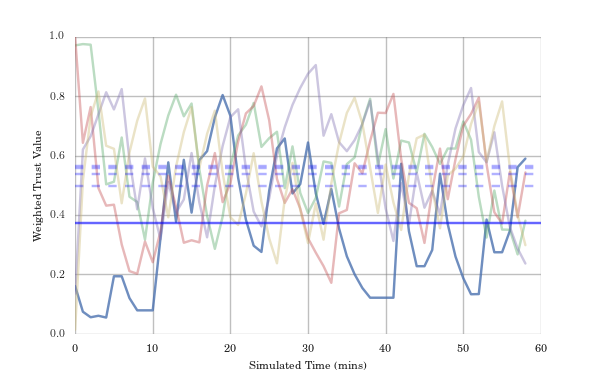
\includegraphics[width=\linewidth]{best_comms_run_STS}
	\caption{Selfish(STS) Targeting Comms Metric Trust}
	\label{fig:comms_sts}
\end{figure}

\begin{figure}[h]
	\centering
	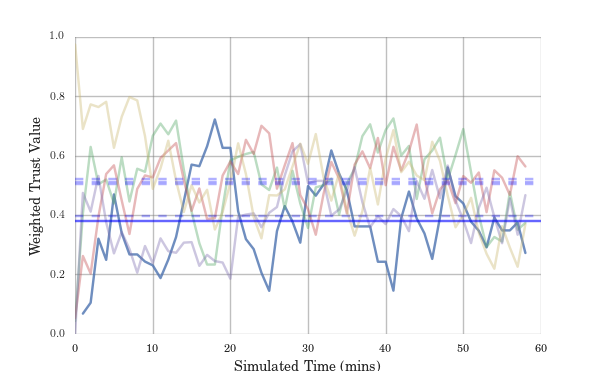
\includegraphics[width=\linewidth]{best_full_run_STS}
	\caption{Selfish(STS) Targeting Full Metric Trust}
	\label{fig:full_sts}
\end{figure}

\begin{figure}[h]
	\centering
	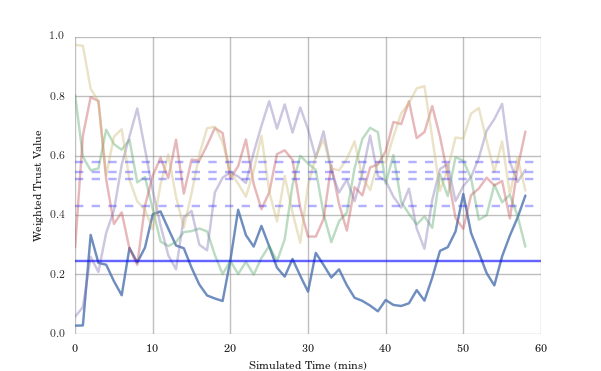
\includegraphics[width=\linewidth]{best_comms_run_Shadow}
	\caption{Shadow Comms Metric Trust}
	\label{fig:comms_shadow}
\end{figure}

\begin{figure}[h]
	\centering
	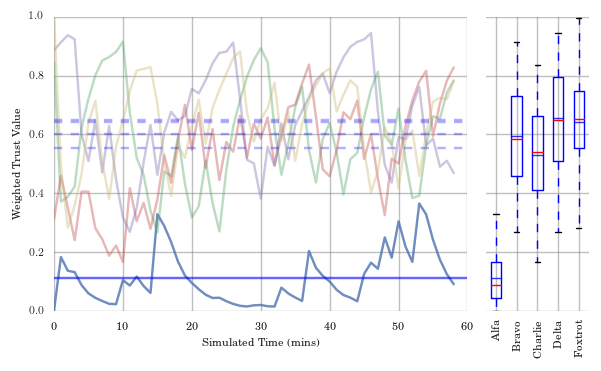
\includegraphics[width=\linewidth]{best_full_run_Shadow}
	\caption{Shadow Full Metric Trust}
	\label{fig:full_shadow}
\end{figure}


\begin{figure}[h]
	\centering
  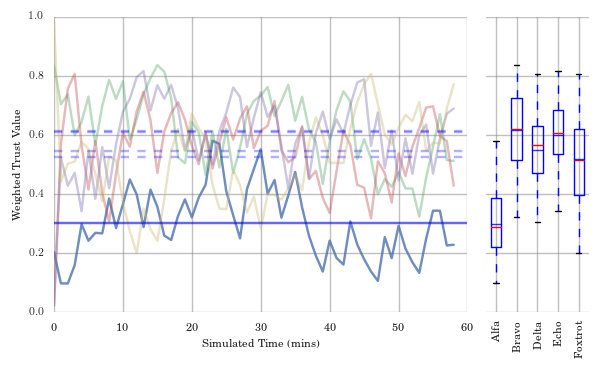
\includegraphics[width=\linewidth]{best_comms_run_SlowCoach}
	\caption{SlowCoach Comms Metric Trust}
	\label{fig:comms_slowcoach}
\end{figure}


\begin{figure}[h]
	\centering
  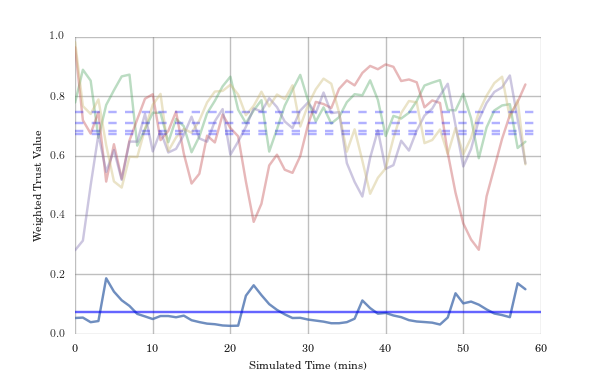
\includegraphics[width=\linewidth]{best_full_run_SlowCoach}
	\caption{SlowCoach Full Metric Trust}
	\label{fig:full_slowcoach}
\end{figure}


\begin{table}
\centering
\caption{$\Delta T$ across domains and detected behaviours}
\begin{tabular}{|l|r|r|r|r|r|}
\hline
Behaviour &       MPC &       STS &    Shadow & SlowCoach & Avg.\\
\hline
Domain &           &           &           &           &\\
Full   &  0.905 &  0.101 &  0.499 &  0.627 & 0.533\\
Comms  &  0.954 &  0.166 &  0.287 &  0.268 & 0.419 \\
Phys   &  0.022 &  0.020 &  0.421 &  0.756 & 0.305\\
\hline
Avg.   &  0.627 &  0.096 &  0.402 &  0.550 &  0.419 \\
\hline
\end{tabular}
\label{tab:domain_deltas}
\end{table}

\section{Conclusion}
In this paper we demonstrate that in harsh environments, multi-domain trust assessment can perform better on average than single-domain counterparts, both in terms of robustness and sensitivity, but also covering a wider region of the potential behaviour space, 

The extension of the methodologies of multi-vector trust into the marine space are already demonstrated, however including information from physical observations of actors in a network enables the detection and identification of a much wider range of behaviours.
We also demonstrate a method for assessing trust metrics in harsh environments in terms of their relative significance, and a method for establishing classification signatures for misbehaviours.

It is to be noted that this presented method is significantly more computationally intensive than the relatively simple Hermes / OTMF algorithms communications only algorithms, and is exponential in complexity as metrics and/or domains are added. The repeated metric re-weighting required for real time behaviour detection is therefore an area that requires optimization. More work needs to be done to characterise how worthwhile this approach is compared to a separate synthesis approach where by MTFM-style trust is generated and assessed on a per-domain basis and subsequently fuzed.

For greater fidelity and more optimal results, a wider range of weights can be used in the initial regression step; however this is computationally expensive given that weighting is applied to each perspective (i.e. observer/target node pair) for each trust assessment time step, presenting 15 perspectives at each time interval in the 6 node case.

Every effort has been made to avoid over-training the dataset, using cross validating sampling for regression and "best weight" generation, however more meta-analysis is required to further demonstrate the functionality of this process.



%%%%%%%%%%%%%%%%%%%%%%%%%%%%%%%%%%%%%%%%%%%%%%%%%%%%%%%%%%%%%%%%%%%%%%%%%%%%%%%
\ifx\ifthesis\undefined
	%% ----------------------------------------------------------------
\label{Bibliography}
% \bibliographystyle{amsplain}
%\bibliographystyle{unsrtnat}  % Use the "unsrtnat" BibTeX style for formatting the Bibliography
\bibliographystyle{alpha}
\bibliography{../Thesis}  % The references (bibliography) information are stored in the file named "Thesis.bib"

\end{document}  % The End
%% ----------------------------------------------------------------
\else
\fi
